%        File: sheet.tex
%     Created: Mon Mar 14 04:00 PM 2016 C
%
\documentclass[a4paper,twocolumn]{article}

\usepackage{geometry}
\usepackage{amsmath}
\usepackage{amssymb}
\usepackage{graphicx}
\usepackage{float}
\usepackage{appendix}

\geometry{a4paper, margin={.3in, .3in}}

\title{Computer Vision 1 - Cheat Sheet}
\author{Andrea Jemmett}

\begin{document}
\maketitle

\section{Color Models}
Color is part of the electromagnetic spectrum with energy in the range from 380
to 780 nm wavelength. Most of the colors we perceive are a mixture of
wavelengths where the amount of energy at each wavelength is given by the
spectral energy distribution (SED). When white light shines upon an object, some
wavelengths are absorbed and other are reflected (a green object will reflect
light with wavelength around 500nm, other wavelengths will be absorbed). The
\textbf{hue} corresponds with the dominant wavelength of the SED;
\textbf{saturation} is defined as the proportion of pure light with respect to
white light needed to produce the color; \textbf{lightness} is the intensity of
the reflected light meanwhile \textbf{brightness} is the intensity of the light
source. Let $EH$ be the dominant wavelength in the SED and $EW$ the wavelength
contributing to the white light, then the \textit{hue} is equal to $EH$, the
\textit{saturation} equals to the difference $EH - EW$ and the
\textit{lightness} equals to the area underlined by the SED.

\begin{figure}[htpb]
	\centering
	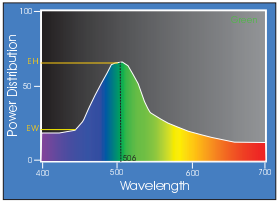
\includegraphics[height=1.5in]{imgs/color-sed.png}
\end{figure}

Experiments have been conducted in which a human observer was asked to adjust
three knobs which control the intensity of a three primary colors so to match
the (perceived) color of the test light. The three primary lights were
additively mixed in and the knobs' values were recorded yielding the so called
color matching functions $\bar{r}(\lambda)$, $\bar{g}(\lambda)$ and
$\bar{b}(\lambda)$. The problem with these was that a negative amount of
at least one of the primaries was necessary to produce the full spectra. So the
CIE proposed a mathematical transformation, the \textbf{XYZ} model, which uses
another set of color matching functions: $\bar{x}(\lambda)$, $\bar{y}(\lambda)$
and $\bar{z}(\lambda)$.

The observer perceives color in terms of three color signals based on the
trichromacy theory and can be modeled as:
\begin{equation} \label{eq:color-perception}
C = \int_{\lambda} E(\lambda) S(\lambda) f_C(\lambda) d\lambda
\end{equation}
where $C \in \{R, G, B\}$, $E$ is the SPD, $S$ is the light reflected by objects
and $f_C$ is the color matching function. If we use $\bar{x}$, $\bar{y}$ and
$\bar{z}$ then we have the XYZ color space. To better represent graphically this
color space we can compute the $xyz$ values as follows:
\begin{equation}
x = \frac{X}{X + Y + Z} \quad y = \frac{Y}{X + Y + Z} \quad z = \frac{Z}{X + Y + Z}
\end{equation}
where we factor out the intensity. Since the chromaticity values sum to unity,
two elements are sufficient to represent a color. When the $x$ and $y$ values
are represented on a plane the chromaticity diagram is obtained. We can also
infer the hue from the chromaticity diagram: first we need to select a reference
white light, the hue is then the wavelength at the spectral curve that
intersects the line from reference light through the color point to the spectral
curve (this point is $G_2$). If $||G_1||$ is the distance from the color to the
white light and $||G_2||$ is the distance from $G_2$ to the white source, then
the saturation is given by $\frac{||G_1||}{||G_2||}$.

RGB values can be obtained using equation \ref{eq:color-perception} and the
$\bar{r}$, $\bar{g}$, and $\bar{b}$ color matching functions. The projection of
RGB points on the rgb chromaticity triangle is defined by:
\begin{equation}
r = \frac{R}{R + G + B} \quad g = \frac{G}{R + G + B} \quad b = \frac{B}{R + G + B}
\end{equation}
In the HSI chromaticity diagram, we compute hue and saturation in the following
way: by assuming white light we define a reference point of $r = g = b = 1/3$,
the saturation can than be computed as:
\begin{equation}
S_{rgb}(r, g, b) = \sqrt{(r - 1/3)^2 + (g - 1/3)^2 + (b - 1/3)^2}
\end{equation}
or
\begin{equation}
S(R, G, B) = 1 - \frac{min(R, G, B)}{R + G + B}
\end{equation}
while the hue is given by:
\begin{equation}
H_{rgb}(r, g, b) = arctan(\frac{r - 1/3}{g - 1/3})
\end{equation}
or
\begin{equation}
H(R, G, B) = arctan(\frac{\sqrt{3}(G - B)}{(R - G) + (R - B)})
\end{equation}

A color invariant system contains color invariant models that are more or less
insensitive to the varying image conditions. For matte surfaces
\textit{RGB} is sensitive to orientation while \textit{rgb} is (assuming
constant white light) insensitive to orientation, illumination direction and
intensity (similarly are S and H). For shiny surfaces H is color invariant.


\section{Surface Reflection}
The Bidirectional Reflectance Distribution Function (BRDF) is the most general
model of light scattering. Describes how much light arriving at an incident
direction $\mathbf{v_i}$ is emitted in a reflected direction $\mathbf{v_r}$. It
can be written as a function of the angles of incident and reflected light like so:
\begin{equation}
f_{BRDF}(\theta_i, \phi_i, \theta_r, \phi_r) =
	\frac{radiance\_of(\theta_r, \phi_r)}{irradiance\_at(\theta_i, \phi_i)}
\end{equation}
Typically BRDF can be split into \textit{diffuse} and \textit{specular}
components. The \textbf{diffuse} component (\textit{Lambertian} or \textit{matte}
reflection) scatters light uniformly in all directions and is associated with
the phenomena of \textit{shading}. Light is scattered uniformly across all
directions (the BRDF is constant):
\begin{equation}
f_d(\theta_i, \phi_i, \theta_r, \phi_r) = \frac{\rho_d}{\pi}
\end{equation}
but the amount of light depends on the angle between the incident direction and
the surface normal $\theta_i$ (is independent of the viewing direction
$\mathbf{v}$):
\begin{equation}
radiance\_of_d = \frac{\rho_d}{\pi} I cos(\theta_i)
\end{equation}
where $\rho_d$ is the surface albedo and $I$ is the source intensity.
This is because the surface area exposed to a given amount of light becomes
larger at oblique angles. The \textbf{specular} (glossy or highlight) BRDF reflection
depends strongly on the outgoing light direction. All the incident light energy
is reflected in a \textit{single} direction (only when $v_i = v_r$). So the
mirror BRDF is a delta function:
\begin{equation}
f_s(\theta_i, \phi_i, \theta_v, \phi_v) = \rho \delta(\theta_i - \theta_v)
\delta(\phi_i + \pi - \phi_v)
\end{equation}
\begin{equation}
radiance\_of_s = I f_d(\theta_i, \phi_i, \theta_v, \phi_v)
\end{equation}

Another reflectance model is the \textbf{Phong} model which uses an
\textit{ambient illumination} component besides diffuse and specular.


\section{Image Processing}
We can think of an image as a function from $\mathbb{R}^2$ to $\mathbb{R}$.

\subsection{Point Operators}
Act on a single point, that is locality in the image is lost.
\paragraph{Contrast and Brightness} also called \textit{gain} and
\textit{bias} are defined by the following operation:
\begin{equation}
g(\mathbf{x}) = a f(\mathbf{x}) + b
\end{equation}
where $a$ and $b$ are gain and bias respectively.
\paragraph{Gamma Correction} is used to remove the non-linear mapping between
the input radiance and the pixel values (invert gamma mapping):
\begin{equation}
g(\mathbf{x}) = [f(\mathbf{x})]^{\frac{1}{\gamma}}
\end{equation}
where $\gamma = 2.2$ is a reasonable fit for most cameras.
\paragraph{Histogram Equalization} is used to transform an image so that the
resulting histogram is flat. A pro of this is that we can show the entire color
range, but a flat histogram results in a muddy-looking picture. A solution to
this is to perform a \textit{partial} histogram equalization, that is blend the
full histogram equalization and an identity transform.

\subsection{Neighborhood Processing (Filtering)}
Act on a neighborhood of pixels, that is spatial information is preserved.
\subsubsection{Linear Filters}
This class of filters have the property of being linear (the response to the sum
of two signals is equal to the sum of the responses of the two signals
separately). It could be formulated as follows:
\begin{equation}
g(i, j) = \sum_{k,l} h(k, l) f(i + k, j + l)
\end{equation}
and is called a \textit{correlation}. A common variant is the following:
\begin{equation}
g(i, j) = \sum_{k,l} h(k, l) f(i - k , j - l)
\end{equation}
and is called a \textit{convolution}. Note that a filter correlated with an
image returns the flipped image, whereas the result of a convolution has the
same orientation because the sign of the offsets have been reversed.

Linear filters suffer from boundary effects, this is because the original image
is being padded with zero valued pixels wherever the convolution kernel extends
beyond the image boundaries. There exist a number of padding techniques:
\textit{zero} sets all pixels outside the image with zeros, \textit{constant}
sets all pixels to a specified border color, \textit{clamp} repeats edge pixels
indefinitely, \textit{cyclic} wraps pixels around the image and \textit{mirror}
reflected pixel along the edge.

\paragraph{Separable filtering}
The cost of performing a convolution is of $K^2$ operations per pixel. This
operation can be sped up by performing first a 1D horizontal and then vertical
convolution. This results in $2K$ operations per pixel. A kernel for which this
is possible is said to be \textit{separable}. So a 2D kernel $\mathbf{K}$ is
equal to the outer product of two 1D filters
$\mathbf{K}=\mathbf{v}\mathbf{h}^T$ in vertical and horizontal directions.
Determining if a kernel is separable is often done by inspection, using the
analytical form or using SVD.

\subsubsection{Common linear filters}
\paragraph{Box or moving average} simply takes the average in a $K^2$ window so has
	a smoothing effect; it's equal to convolving with a kernel of all ones
	and then scaling; for example:
	\begin{equation}
		\frac{1}{9} \quad \begin{bmatrix}
			1 & 1 & 1 \\
			1 & 1 & 1 \\
			1 & 1 & 1
		\end{bmatrix}
	\end{equation}
\paragraph{Sharpening} accentuate difference with local average:
	\begin{equation}
		\begin{bmatrix}
			0 & 0 & 0 \\
			0 & 2 & 0 \\
			0 & 0 & 0
		\end{bmatrix}
		\quad - \quad \frac{1}{9} \quad \begin{bmatrix}
			1 & 1 & 1 \\
			1 & 1 & 1 \\
			1 & 1 & 1
		\end{bmatrix}
	\end{equation}
\paragraph{Sobel} used to find edges in one direction:
	\begin{equation}
		\begin{bmatrix}
			-1 & -2 & -1 \\
			 0 &  0 &  0 \\
			 1 &  2 &  1
		\end{bmatrix}
	\end{equation}
	finds horizontal edges;
\paragraph{Gaussian} weights contribution of pixels by their nearness, so has a
	smoothing effect;
	\begin{equation}
		G_{\sigma} = \frac{1}{2\pi\sigma^2}e^{-\frac{x^2+y^2}{2\sigma^2}}
	\end{equation}
	the parameter $\sigma$ is a smoothing parameter, larger $\sigma$ corresponds
	to a blurrier image; removes high-frequency components and so acts as a
	low-pass filter; it is a \textit{separable} kernel; used to denoise Gaussian
	additive noise (not salt and pepper);
\paragraph{Laplacian of Gaussian} is a \textit{steerable} filter defined as:
	\begin{equation} \label{eq:log}
		\nabla^2 G = \frac{\partial G}{\partial x} + \frac{\partial G}{\partial y}
		= \left(\frac{x^2 + y^2}{\sigma^4} - \frac{2}{\sigma^2}\right) G
	\end{equation}

\subsubsection{Non-linear Filters}
In many case better performance can be achieved using a \textit{non-linear}
combination of pixels instead of a weighted average, as in linear filters. For
example in case of shot noise a Gaussian filter would result in the noisy pixels
being softened instead of removed.
\paragraph{Median filter} uses the median value from the pixel's neighborhood;
it's effective against shot noise because noisy pixel value usually lie away from
the true value in the neighborhood;
\paragraph{Bilateral filtering} the output pixel value depends on a weighted
combination of neighbour pixel values; weights are determined using both spatial
distance and intensity difference.


\section{Feature Extraction}
There are two kind of features. The first are \textbf{keypoint features} (interest points,
corners) and are single points on the image and are
characterized by their neighborhood using a \textit{descriptor}; these interest
points can then be matched in two different images to successively align them
for example. The feature matching pipeline is as follows:
\begin{enumerate}
  \item find a set of distinctive keypoints;
  \item define a region around each point;
  \item extract and normalize the region content;
  \item compute a local descriptor for each region;
  \item match local descriptors.
\end{enumerate}
It is important for keypoint features to be \textit{repeatable} and
\textit{distinctive}; also they need to be \textit{invariant} to translation,
rotation, scaling and other imaging parameters.
The second kind of features are \textbf{edges} that are used to get
orientation and local appearence of an object.

\subsection{Edge Detectors}
Edges are caused by a variety of factors, mostly discontinuities. For example
surface normal (change in shape), depth (objects at different perspective
levels), surface color (some lettering on a label) or illumination (shadows).
Analytically an edge is a rapid change in the image function. To find these
rapid changes we can apply a derivative to a signal so that the extrema of the
resulting signal are the rapid changes of the original input signal. If we apply
the derivation directly on the image we will obtain a noisier image back. To
cope with this we need to smooth the image first by applying a Gaussian filter.
Because both convolution and differentiation are linear operators they commute
so that we can write
\begin{equation}
	\mathbf{J_{\sigma}} = \nabla (G_{\sigma} * I) = \nabla (G_{\sigma}) * I = G_{\sigma} * \nabla(I)
\end{equation}
and this simplifies the edge detection operator because we could reuse a
derivative of Gaussian for multiple images without ever computing the actual
image derivative. This is often called a \textit{Derivative of Gaussian} filter.
The $\sigma$ in this case determines the scale at which the filter is going to
find edges, but may also blur the edges too much.

\subsubsection{Canny Edge Detector}
The Canny operator transforms an input image into a binary edge map of thin
(having width of one pixel) edge segments. The first step is to compute the
\textit{image gradient} in the $x$ and $y$ directions. We can use the Sobel
operator, that provides an approximation of the partial derivatives, or the DoG.
Then from the image gradients $I_x$ and $I_y$ we can compute the
\textit{orientation} as $\theta = atan2(I_x, I_y)$ and round it to multiplies of
$\pi/4$. A step of \textit{non-maxima suppression} is employed to test whether a
gradient value $g(p)$ is maximal in the direction given by $\theta(p)$.
The final step is edge linking (or \textit{hysteresis}). By using two thresholds
$T_{low}$ and $T_{high}$ we link edgels found where $g(p) \ge T_{high}$ with
edgels $q$ found in its neighborhood where $g(q) \ge T_{low}$. Another parameter
that controls the results of the operator is the $\sigma$ in case of DoG; small
$\sigma$ means fine features, large $\sigma$ detects large scale edges.

\subsection{Blob Detectors}
Blob detection methods aim at detecting regions in an image that differ in
properties (brightness, color) comparing to surrounding regions; all points in a
blob can be considered in some sense similar to each other.

\subsubsection{Laplacian of Gaussian}
The LoG is defined by the Laplacian operator applied to a Gaussian kernel
(\ref{eq:log}) and is a circularly symmetric kernel suitable for blob detection.
With this operator edges are identified by its zero-crossings.
\begin{figure}[htpb]
				\centering
				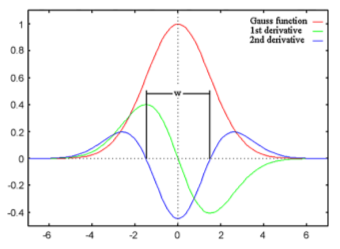
\includegraphics[height=1.5in]{imgs/gauss-profile.png}
\end{figure}
It is possible to build a \textit{pyramid} of Laplacians in the \textit{scale
space} by applying the LoG operator repeatedly with different scales (controlled
by $\sigma$) so to obtain different layers of Laplacian responses that may be
used to identify blobs at different scales. We define the \textit{characteristic
scale} as the scale that produces the highest peak of Laplacian response.

\subsection{Color Edge Detection and Classification}
While most edge detectors have been developed for grayscale images, color images
can provide useful information. For example edges between iso-illuminants
(colors that have the same illuminance) fail to be detected by grayscale edge
operators. A simple approach is to combine outputs of grayscale detectors
applied to each color band separately. A better approach is to compute the
\textit{oriented energy} in each channel (by using a steerable filter like DoG
or LoG), compute the gradient by summing gradient magnitudes separately:
\begin{equation}
	|\nabla C(x, y)| = \sqrt{R_x^2 + R_y^2} + \sqrt{G_x^2 + G_y^2} + \sqrt{B_x^2 + B_y^2}
\end{equation}
or using the Euclidean metric:
\begin{equation}
	|\nabla C(x,y)| = \sqrt{R_x^2 + R_y^2 + G_x^2 + G_y^2 + B_x^2 + B_y^2}
\end{equation}
or using eigenvalues.

We can use different gradients with different color spaces
to \textbf{classify} edges as being \textit{color edges}, \textit{shadows} or
\textit{highlights}. We need first to compute the color gradient in two color
spaces, one invariant to matte surfaces and one to shiny surfaces, such as
\textit{rgb} and \textit{Hue}, and define two thresholds $t_{rgb}$ and $t_H$.
Then if $|\nabla C_{rgb}| \ge t_{rgb} \wedge |\nabla C_H| < t_H$ we classify as
highlight edge, else if $|\nabla C_H| \ge t_H$ classify as color edge else
classify as shadow edge. An application of this technique is \textit{shadow removal}.
First we classify shadow edges in each color band, then the image is separated
into invariant and shadow image and the latter is subtracted (in log space) from
the original image.

\subsection{Harris Corner Detector}
We can distinguish different kind of structures for features, based on their
dimensionality; at 0D we have single points that are not useful for matching; at
1D we found edges that can be localized in 1D, that is we can move along the
edge; at 2D we can localize \textit{corners}, that is we can identify a feature
by moving along two directions, finding a corner. This issue is commonly called
\textit{aperture problem}. These ideas can be formalized using the simplest
possible matching criterion between two image patches, the sum of square
differences (SSD):
\begin{equation} \label{eq:ssd}
	E_{SSD}(u,v) = \sum_i w(x_i,y_i) [I_1(x+u,y+v) - I_0(x,y)]^2
\end{equation}
where $I_0$ and $I_1$ are two images being compared, $w$ is a window,
$\mathbf{u} = [u, v]$ and the summation is over all pixels in the patch (note
that this is the same formulation for Optical Flow estimation).

Because we don't know which other image locations the feature will end up being
matched against, we can only compute the so called \textit{auto-correlation}
comparing an image patch with itself with respect to small variations $\Delta\mathbf{u}$:
\begin{equation}
	E_{AC}(\Delta u, \Delta v) = \sum_i w(x_i,y_i) [I(x+\Delta u, y+\Delta v) - I(x,y)]^2
\end{equation}
Using a Taylor Series expansion of the image function $I(\mathbf{x_i}+\Delta
\mathbf{u} \equiv I(\mathbf{x_i}) \nabla I(\mathbf{x_i})\Delta \mathbf{u}$ we
can approximate the auto-correlation surface as:
\begin{equation}
	E_{AC}(\Delta \mathbf{u})=\Delta \mathbf{u}^T \mathbf{A} \Delta \mathbf{u}
\end{equation}
where
\begin{equation}
	\mathbf{A} = w * \begin{bmatrix}
		I_x^2 & I_x I_y \\
		I_x I_y & I_y^2
	\end{bmatrix}
\end{equation}
and $I_x$ and $I_y$ represents gradients in $x$ and $y$ directions. If we
consider a single pixel $\mathbf{p}$, we can define
\begin{equation}
	\mathbf{G_p} = \begin{bmatrix}
		I_x^2(\mathbf{p}) & I_x(\mathbf{p}) I_y(\mathbf{p}) \\
		I_x(\mathbf{p}) I_y(\mathbf{p}) & I_y^2(\mathbf{p})
	\end{bmatrix}
\end{equation}
This pixel is a corner feature if the eigenvalues $\lambda_1$ and $\lambda_2$
are both large and of similar magnitude. We can define the \textit{cornerness
measure} as
\begin{equation}
	H(\mathbf{p}) = det(\mathbf{G_p}) - \alpha Tr(\mathbf{G_p})
\end{equation}
with $0.04 \le \alpha \le 0.06$. Due to the properties of eigenvalues we can
write
\begin{equation}
	H(\mathbf{p}) = \lambda_1 \lambda_2 - \alpha (\lambda_1 + \lambda_2)
\end{equation}
The response function $H$ depends on the eigenvalues of $A$ so that if it is
large there is a corner, is negative with large magnitude for an edge and
$|H|$ is small for a flat region.

\paragraph{Harris Corner Detector algorithm}
\begin{enumerate}
	\item Compute $x$ and $y$ derivatives of image
		$$I_x=G_{\sigma}^x * I \qquad I_y = G_{\sigma}^y * I$$
	\item Compute product of derivatives pixel-wise to build matrix $\mathbf{A}$
	\item Convolve each of these images with a larger Gaussian
	\item Build a matrix $\mathbf{G}$ for each pixel
	\item Compute the cornerness measure $H$ for each pixel
	\item Threshold on values of $H$ and compute non-maxima suppression
\end{enumerate}


\subsection{Template Matching}
The goal is to find an image template inside a bigger image (scene). There are
two methods. The first one consists in using a SSD (eq. \ref{eq:ssd}) that signals how much the
template differ from the examined window around a pixel. Because of this we need
to take a $1 - \sqrt{SSD}$ to than identify the maxima as true detections.
A second approach consists in using the normalized cross-correlation as
\begin{equation}
	h[m,n]=\frac{\sum_{k,l}(g[k,l]-\bar{g})(f[m-k,n-l]-\bar{f}_{m,n})}
		{\sqrt{\sum_{k,l}(g[k,l]\bar{g})^2\sum_{k,l}(f[m-k,n-l]-\bar{f}_{m,n})^2}}
\end{equation}
where $\bar{g}$ is the mean template and $\bar{f}_{m,n}$ is the mean image patch.
The normalized cross-correlation responds positively for similar patches, so we
can apply a thresholding operation directly on it to find the template.

SSD is usually faster but is sensitive to the overall intensities. Normalized
cross-correlation methods instead are slower but invariant to local average
intensity and contrast.



\newpage

\begin{appendices}
	\section{Linear Algebra}
	\paragraph{Trace} of a $n \times n$ matrix $\mathbf{A} = (a_{ij})$:
	\begin{equation}
		Tr(\mathbf{A}) = \sum_{i=1}^n a_{ii}
	\end{equation}
	\paragraph{Determinant} of a $2 \times 2$ matrix $\mathbf{A} = (a_{ij})$ is:
	\begin{equation}
		det(\mathbf{A}) = a_{11} a_{22} - a_{12} a_{21}
	\end{equation}
	for a $3 \times 3$ matrix is:
	\begin{multline*}
		det(\mathbf{A}) = a_{11} a_{22} a_{33} + a_{12} a_{23} a_{31} +
		a_{13} a_{21} a_{32} + \\ - a_{13} a_{22} a_{31} - a_{12} a_{21}
		a_{33} - a_{11} a_{23} a_{32}
	\end{multline*}
	\paragraph{Eigenvalues} of an $n \times n$ matrix $\mathbf{A}$ are the $n$
	solutions to the \textit{characteristic equation} $det(\mathbf{A} - \lambda
	\mathbf{I}) = 0$. The determinant of a square matrix is equal to the product
	of its eigenvalues, and the trace is equal to the sum of the eigenvalues.
\end{appendices}


\end{document}

